\documentclass[a4paper,10pt]{article}

\usepackage{url}
\usepackage{enumerate}
\usepackage{graphicx}
\usepackage{verbatim}


\begin{document}
\title{ARGUS Quick Start Tutorial}

\maketitle

\newpage
\section*{About This Tutorial}
 This tutorial demonstrates basic set-up and design methods available in the web version (\url{kraken.cse.unsw.edu.au:11137}) 
of ARGUS. By the end of the tutorial, you will have a greater understanding of how to
implement and emulate your own processor-based hardware/software system on FPGA using the ARGUS web.

\subsection*{Additional Resources}
To find the way to use git, see the online tutorial of git at:\newline
\url{https://githowto.com/}

\newpage

\section{Getting Started}

\subsection{Software Requirements}
Operating system, web browser, git are required.

\subsection{Hardware Requiremnets}
None.

\subsection{Setting up ARGUS-Software}
\begin{enumerate}
\item Fork the ARGUS-software repository on github at \url{https://github.com/unsw-cse-esl/argus-software}.
\item Clone your repository. Use git command:\\ 
\texttt{git clone \url{git@github.com:[username]/argus-software.git}}
\item Add remote upstream. Use git command:\\
\texttt{git add upstream \url{https://github.com/unsw-cse-esl/argus-software.git}}
\item If you will run simulation at your local machine, set up environment variables for the architecture-specific GNU/GCC tools. These variable names are used in ARGUS-software's scripts for simulation. For example, for simplescalar, set \texttt{SSPATH=/home/foo/bar/pisa}, and
for Leon2/SPARC, set \texttt{L2PATH=/home/foo/bar/leon2}.
\end{enumerate}

\subsection{Setting up ARGUS-Hardware}\label{sec-ARGHW}
\begin{enumerate}
\item Fork the ARGUS-software repository on github at \url{https://github.com/unsw-cse-esl/argus-hardware}.
\item Clone your repository. Use git command:\\ 
\texttt{git clone \url{git@github.com:[username]/argus-hardware.git}}
\item Add remote upstream. Use git command:\\
\texttt{git add upstream \url{https://github.com/unsw-cse-esl/argus-hardware.git}}
\end{enumerate}



\newpage

\section{Overview of ARGUS Design Flow}

\begin{figure}[tb]
\centering
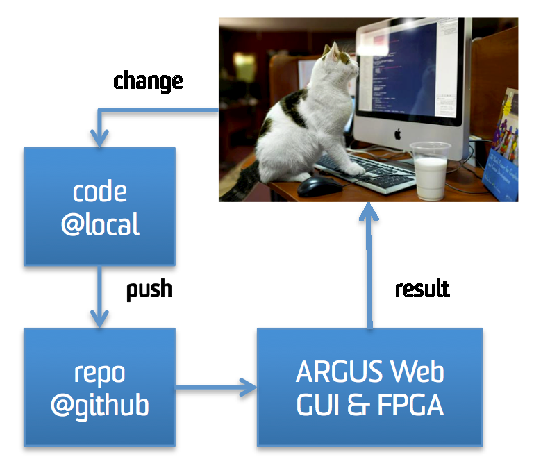
\includegraphics[width=0.6\textwidth]{fig/design-flow.eps}
\caption{Web-based ARGUS Design Flow}\label{fig-designflow}
\end{figure}

Figure~\ref{fig-designflow} shows the basic design flow of using the web-based ARGUS design tool. After the setup of the repository, the user can make changes of the processor hardware or software at local repository. In order to create a FPGA emulation, the user needs to, firstly, \texttt{git commit} and \texttt{git push} the changes (local build) to the github. 

Then, by visiting the website of ARGUS, the user will be able to (1) synthesize the new hardware (ARGUS-hardware flow), and, (2) generate the software on top of the synthesized hardware (ARGUS-software flow). In the end of the software flow, the bitstream containing the entire hardware and software will be automatically transferred to the FPGA, which is connected to the ARGUS server. After the transfer, the FPGA will be automatically configured and emulating the system. The following sections will use an example to go through the entire web-based ARGUS design flow.

\newpage

\section{Creating New ARGUS-Hardware Project}
\begin{figure}[tb]
\centering
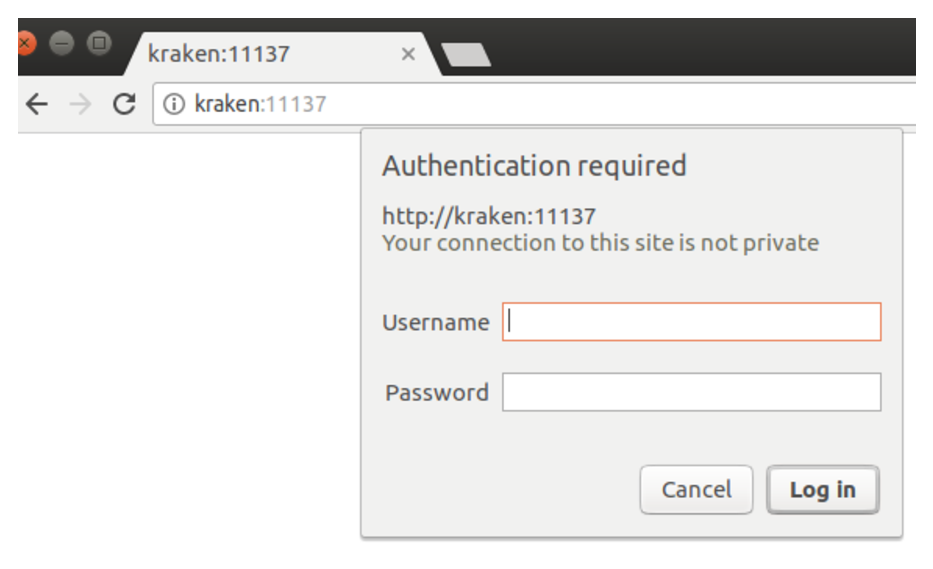
\includegraphics[width=0.6\textwidth]{fig/login.eps}
\caption{Snapshot of authentication page of web ARGUS}\label{fig-login}
\end{figure}•

After ARGUS repository is set up in your machine, you can start to make your own modifications on the processor IPs provided by ARGUS and create the FPGA emulation containing the modified processor in ARGUS. Here we will go through an example ARGUS hardware project as the follows:
\begin{enumerate}
\item Commit and push your modified design to github.
\begin{verbatim}
git add [list of the source files]
git commit -m "description of the commit"
git push
\end{verbatim}•
\item Open ARGUS web GUI in your Internet browser at the address: \texttt{\url{kraken:11137}}. If it is your first time visiting ARGUS web, the authentication page, shown in Figure~\ref{fig-login}, will be seen. Enter your username (ask for username from administrator of ARGUS or Kraken server) in the prompt and click the ``Log in'' button.
\begin{figure}[h]
\centering
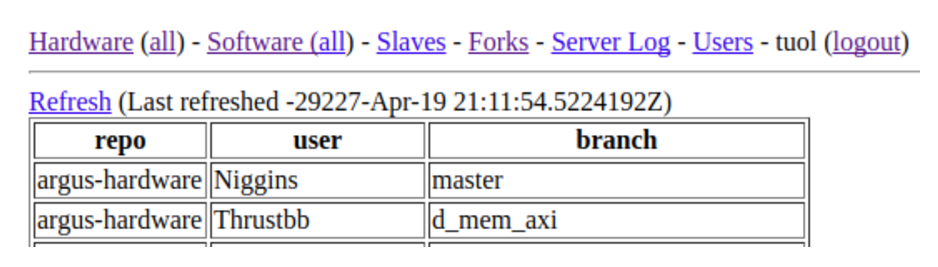
\includegraphics[width=0.7\textwidth]{fig/fork.eps}
\caption{Snapshot of adding new fork}\label{fig-fork}
\end{figure}•
\item As shown in Figure~\ref{fig-fork}, click on the ``Forks'' and then ``Refresh'' in web GUI to let ARGUS add your new github fork (created in Section~\ref{sec-ARGHW}) into the fork list. You might need to wait for a few minutes for this process to be finished.
\begin{figure}[h]
\centering
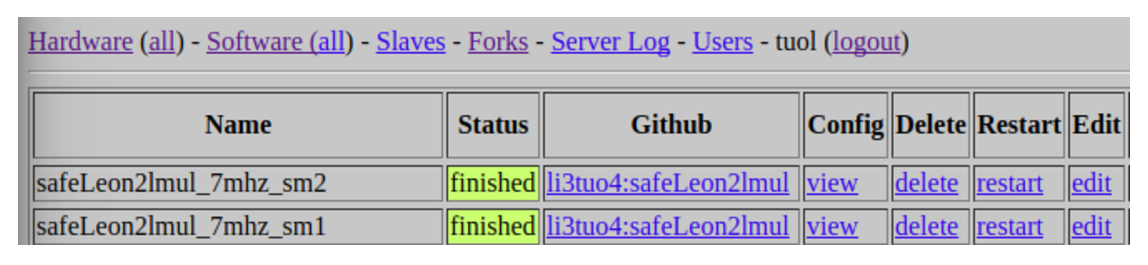
\includegraphics[width=0.7\textwidth]{fig/hwmain.eps}
\caption{Snapshot of ARGUS hardware main page}\label{fig-hwmain}
\end{figure}•
\item Click on the ``Hardware'' and you will see all the hardware projects (see Figure~\ref{fig-hwmain}), which are created by your username in ARGUS. If you would like to see the hardware projects from all the users in ARGUS, click on the ``all'' in the brackets after ``Hardware''. 
\begin{figure}[h]
\centering
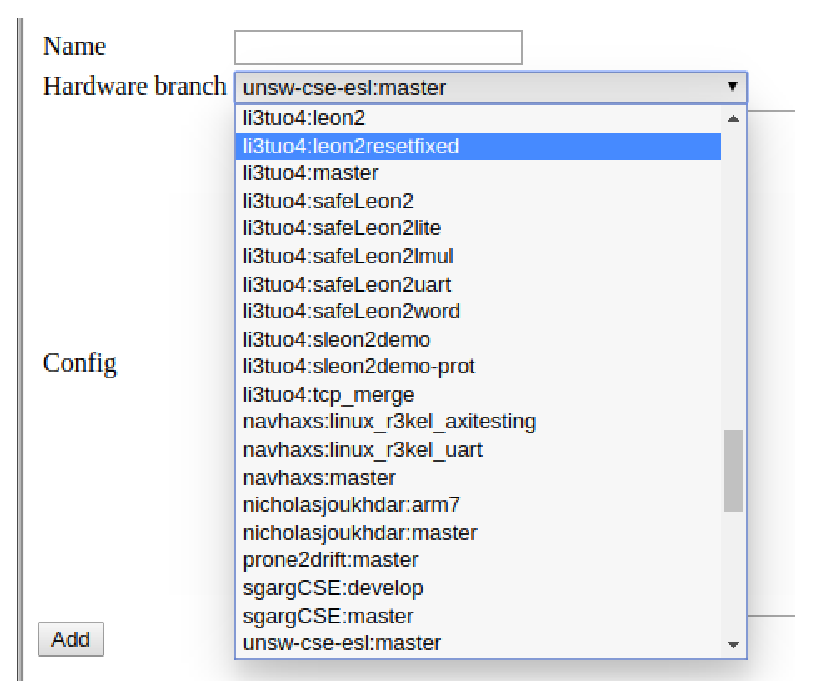
\includegraphics[width=0.7\textwidth]{fig/addhwtask.eps}
\caption{Snapshot of adding ARGUS hardware project}\label{fig-addhwtask}
\end{figure}•
\begin{figure}[h]
\centering
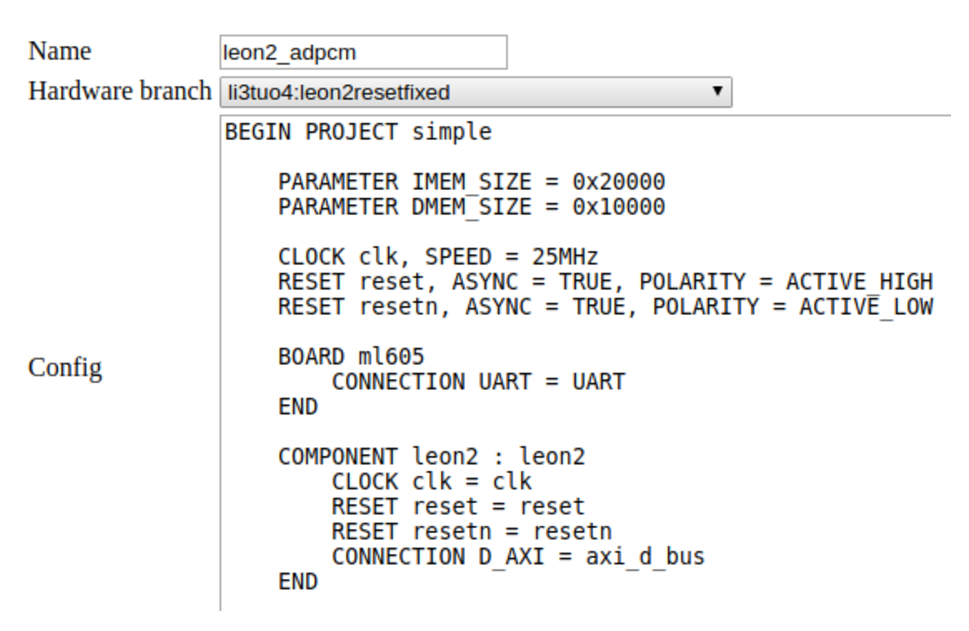
\includegraphics[width=0.7\textwidth]{fig/addhwconfig.eps}
\caption{Snapshot of ARGUS hardware config}\label{fig-addhwconfig}
\end{figure}•
\item Scroll down to the bottom of the page and click on ``Add new task'', and you will see the task specification page, as shown in Figure~\ref{fig-addhwtask}. In this page, select your hardware branch, from the your own fork, which was inserted into ARGUS web at Step 3. Then, type your project name. You also need to fill in the ``Config'', which specifies your hardware. A part of example task config is shown in Figure~\ref{fig-addhwconfig}. If you are new to ARGUS, you can copy the existing config and customize on top of it. At last, click on the ``Add'' button at the leftbottom. 
\item After ``Add'', your new hardware task/project will be read by ARGUS backend and automatically passed to Xilinx ISE for synthesis. You can view the status of the major stages of the synthesis on ARGUS web (need to refresh the webpage by yourself, since ARGUS does not automatically update the status in the current version). If you click on the status in one stage, you can see the detailed runtime log from Xilinx ISE. After the synthesis is finished, the rightmost column (i.e., the last stage ``bit'') will show ``bit''. By clicking on the ``bit'', you can directly download the bitstream of your hardware.

\end{enumerate}•

\newpage

\section{Creating New ARGUS-Software Project}
The first three steps of ARGUS-software flow is same as the ones in ARGUS-hardware flow. The following steps are elabrated as the follows:
\begin{enumerate}
\item Enter the ARGUS software project page by clicking on the ``Software''. Similar to hardware flow, you will see all the software projects created by your username.  If you would like to see the hardware projects from all the users in ARGUS, click on the ``all'' in the brackets after ``Software''.
\begin{figure}[h]
\centering
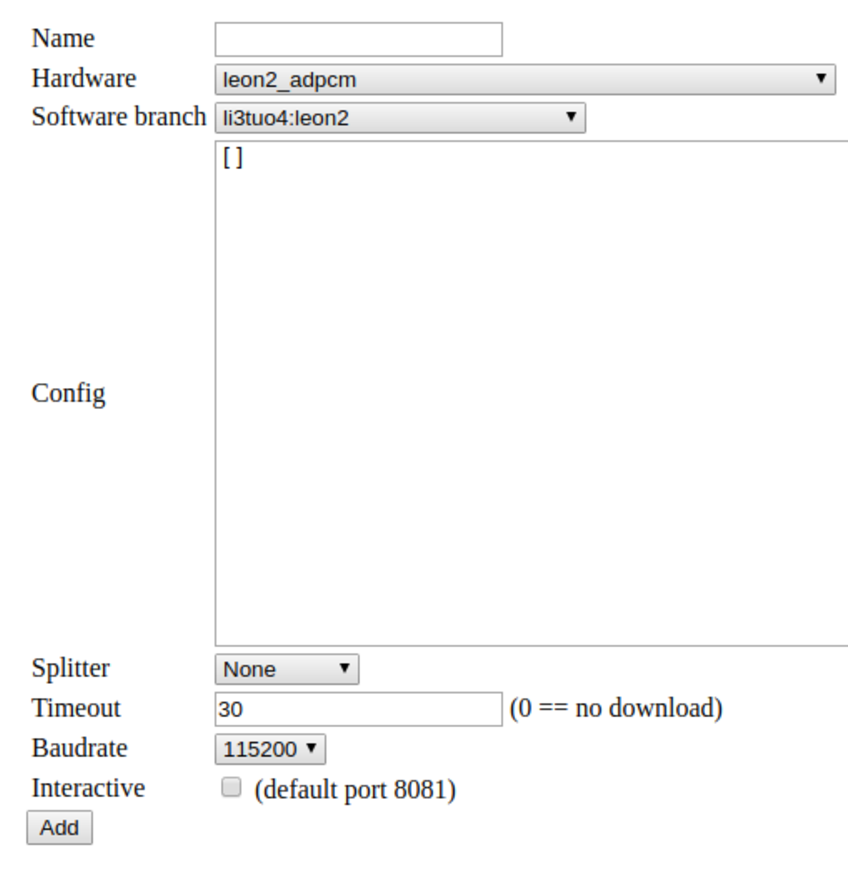
\includegraphics[width=0.7\textwidth]{fig/addswtask.eps}
\caption{Snapshot of adding ARGUS software project}\label{fig-addswtask}
\end{figure}•
\item Scroll down to the bottom of the page and click on ``Add new task'', and you will see the task specification page, as shown in Figure~\ref{fig-addswtask}. Note this page is different to the that of hardware flow. You will need to select both a ``Hardware'' and the ``Software branch''. Select the hardware that has been synthesized in hardware flow. Then, select your software branch, which is pushed from your local machine. Like the hardware flow, you also need to fill in the specification in ``Config''. The following is an example config for Leon2 processor, running ADPCM software.
\begin{verbatim}
[
	{
		"imem": "simple_imem_ctrl",
		"dmem": "simple_dmem_ctrl",
		"name": "simple_leon2",
		"target": "sparcv7w_pg",
		"options": {
			"NODE_NUM": "0"
		},
		"app": "adpcm1"
	}
]
\end{verbatim}•
\item Select ``Splitter''. There are two options, ``Byte'' and ``None'', which decides how the output of the FPGA emulation is shown in the ARGUS web. Usually, None is used. Next, select the timeout time in seconds, since the current version of ARGUS cannot automatically be aware of the completion of the emulation. When timeout is set to 30, ARGUS web will assume the emulation ends after 30 seconds. And, the output of the FPGA at the 30th second will be shown in the last column, which is emulation result. Baudrate is set to 115200. If you want to use ARGUS in interactive mode, you can tickle the box. In this case, the emulation output will not be shown in the ARGUS web. Instead, you will get the output stream at port 8081 of the server called buffalo. 
\item After you finished the previous step, click on the ``Add'' button at the leftbottom. ARGUS will read your task specification, compile the program, generate the system bitstream containing the selected hardware and memory content (i.e., your software build), configure the FPGA with the new bitstream, and collect the emulation output. 
\end{enumerate}•

\newpage

\section{Porting New Processor IP into ARGUS}
Before creating new processor intellectual property (IP) in ARGUS, make sure the steps in Section~\ref{sec-ARGHW} have been done. The major steps are illustrated as the follows:
\begin{enumerate}
\item Enter argus-hardware directory at the local machine.
\begin{verbatim}
cd /path/to/directory/argus-hardware/pcores
\end{verbatim}
\item Create a new directory for your processor IP. In this example, we create a new Leon2 processor, called ``leon2\_v1\_00\_a''.
\begin{verbatim}
mkdir /path/to/directory/argus-hardware/pcores/leon2_v1_00_a
\end{verbatim}•
\item Create two sub-directories, ``data'' and ``hdl'', in the new directory that is just made. 
\begin{verbatim}
mkdir data; mkdir hdl
\end{verbatim}•
\item Suppose your source code is written in VHDL. Create a sub-directory, ``vhdl'', in ``hdl'' and copy your source code of processor IP into ``hdl/vhdl''.
\begin{verbatim}
mkdir hdl/vhdl
cp /path/to/directory/source/*.vhd /path/to/directory/argus-
hardware/pcores/leon2_1_00_a/hdl/vhdl
\end{verbatim}•
\item Go to ``leon2\_v1\_00\_a/data'' and create two new files, ``leon2\_v2\_1\_0.mpd'' and ``leon2\_v2\_1\_0.pao''. The ``.mpd'' file is microprocessor peripheral definition file used by Xilinx ISE, which defines the interface for the peripheral. It mainly includes: (1) ports and default connectivity for bus interfaces; and, (2) parameters and default values. The ``.pao'' file is peripheral analyze order file. It contains a list of Hardware Description Language (HDL) files that are needed for synthesis, and defines the analyze order for compilation. An example mpd file is shown below:
\small
\begin{verbatim}

BEGIN leon2

## Peripheral Options
OPTION IPTYPE = PROCESSOR
OPTION IMP_NETLIST = TRUE
OPTION HDL = MIXED
OPTION IP_GROUP = USER
OPTION ARCH_SUPPORT_MAP = (virtex6 = DEVELOPMENT)

## Bus Interfaces
BUS_INTERFACE BUS = D_AXI, BUS_STD = AXI, BUS_TYPE = MASTER

## Generics for VHDL or Parameters for Verilog
PARAMETER C_D_AXI_PROTOCOL = AXI4, TYPE = NON_HDL, ASSIGNMENT = CONSTANT, 
DT = STRING, BUS = D_AXI
PARAMETER C_D_AXI_ID_WIDTH = 1, ASSIGNMENT = CONSTANT, DT = INTEGER, BUS = D_AXI
PARAMETER C_D_AXI_USER_WIDTH = 1, ASSIGNMENT = CONSTANT, DT = INTEGER, BUS = D_AXI
PARAMETER C_D_AXI_ADDR_WIDTH = 32, ASSIGNMENT = CONSTANT, DT = INTEGER, BUS = D_AXI
PARAMETER C_D_AXI_DATA_WIDTH = 32, ASSIGNMENT = CONSTANT, DT = INTEGER, BUS = D_AXI

## Ports
PORT clk = "", DIR = I, SIGIS = CLK
PORT reset = "", DIR = I, SIGIS = RST
PORT resetn = "", DIR = I, SIGIS = RST

PORT D_AXI_ACLK = "", DIR = I, BUS = D_AXI, SIGIS = CLK, ASSIGNMENT = REQUIRE
PORT D_AXI_ARESETN = ARESETN, DIR = I, BUS = D_AXI, SIGIS = RST

PORT D_AXI_ARID = ARID, DIR = O, VEC = [(C_D_AXI_ID_WIDTH-1):0], BUS = D_AXI
PORT D_AXI_ARADDR = ARADDR, DIR = O, VEC = [(C_D_AXI_ADDR_WIDTH-1):0], BUS = D_AXI
PORT D_AXI_ARLEN = ARLEN, DIR = O, VEC = [7:0], BUS = D_AXI
PORT D_AXI_ARSIZE = ARSIZE, DIR = O, VEC = [2:0], BUS = D_AXI
PORT D_AXI_ARBURST = ARBURST, DIR = O, VEC = [1:0], BUS = D_AXI
PORT D_AXI_ARLOCK = ARLOCK, DIR = O, VEC = [1:0], BUS = D_AXI
PORT D_AXI_ARCACHE = ARCACHE, DIR = O, VEC = [3:0], BUS = D_AXI
PORT D_AXI_ARPROT = ARPROT, DIR = O, VEC = [2:0], BUS = D_AXI
PORT D_AXI_ARREGION = ARREGION, DIR = O, VEC = [3:0], BUS = D_AXI
PORT D_AXI_ARQOS = ARQOS, DIR = O, VEC = [3:0], BUS = D_AXI
PORT D_AXI_ARUSER = ARUSER, DIR = O, VEC = [(C_D_AXI_USER_WIDTH-1):0], BUS = D_AXI
PORT D_AXI_ARVALID = ARVALID, DIR = O, BUS = D_AXI
PORT D_AXI_ARREADY = ARREADY, DIR = I, BUS = D_AXI

PORT D_AXI_RID = RID, DIR = I, VEC = [(C_D_AXI_ID_WIDTH-1):0], BUS = D_AXI
PORT D_AXI_RDATA = RDATA, DIR = I, VEC = [(C_D_AXI_DATA_WIDTH-1):0], BUS = D_AXI
PORT D_AXI_RRESP = RRESP, DIR = I, VEC = [1:0], BUS = D_AXI
PORT D_AXI_RLAST = RLAST, DIR = I, BUS = D_AXI
PORT D_AXI_RUSER = RUSER, DIR = I, VEC = [(C_D_AXI_USER_WIDTH-1):0], BUS = D_AXI
PORT D_AXI_RVALID = RVALID, DIR = I, BUS = D_AXI
PORT D_AXI_RREADY = RREADY, DIR = O, BUS = D_AXI

PORT D_AXI_AWID = AWID, DIR = O, VEC = [(C_D_AXI_ID_WIDTH-1):0], BUS = D_AXI
PORT D_AXI_AWADDR = AWADDR, DIR = O, VEC = [(C_D_AXI_ADDR_WIDTH-1):0], BUS = D_AXI
PORT D_AXI_AWLEN = AWLEN, DIR = O, VEC = [7:0], BUS = D_AXI
PORT D_AXI_AWSIZE = AWSIZE, DIR = O, VEC = [2:0], BUS = D_AXI
PORT D_AXI_AWBURST = AWBURST, DIR = O, VEC = [1:0], BUS = D_AXI
PORT D_AXI_AWLOCK = AWLOCK, DIR = O, VEC = [1:0], BUS = D_AXI
PORT D_AXI_AWCACHE = AWCACHE, DIR = O, VEC = [3:0], BUS = D_AXI
PORT D_AXI_AWPROT = AWPROT, DIR = O, VEC = [2:0], BUS = D_AXI
PORT D_AXI_AWREGION = AWREGION, DIR = O, VEC = [3:0], BUS = D_AXI
PORT D_AXI_AWQOS = AWQOS, DIR = O, VEC = [3:0], BUS = D_AXI
PORT D_AXI_AWUSER = AWUSER, DIR = O, VEC = [(C_D_AXI_USER_WIDTH-1):0], BUS = D_AXI
PORT D_AXI_AWVALID = AWVALID, DIR = O, BUS = D_AXI
PORT D_AXI_AWREADY = AWREADY, DIR = I, BUS = D_AXI

PORT D_AXI_WID = WID, DIR = O, VEC = [(C_D_AXI_ID_WIDTH-1):0], BUS = D_AXI
PORT D_AXI_WDATA = WDATA, DIR = O, VEC = [(C_D_AXI_DATA_WIDTH-1):0], BUS = D_AXI
PORT D_AXI_WSTRB = WSTRB, DIR = O, VEC = [(C_D_AXI_DATA_WIDTH/8)-1:0], BUS = D_AXI
PORT D_AXI_WLAST = WLAST, DIR = O, BUS = D_AXI
PORT D_AXI_WUSER = WUSER, DIR = O, VEC = [(C_D_AXI_USER_WIDTH-1):0], BUS = D_AXI
PORT D_AXI_WVALID = WVALID, DIR = O, BUS = D_AXI
PORT D_AXI_WREADY = WREADY, DIR = I, BUS = D_AXI

PORT D_AXI_BID = BID, DIR = I, VEC = [(C_D_AXI_ID_WIDTH-1):0], BUS = D_AXI
PORT D_AXI_BRESP = BRESP, DIR = I, VEC = [1:0], BUS = D_AXI
PORT D_AXI_BUSER = BUSER, DIR = I, VEC = [(C_D_AXI_USER_WIDTH-1):0], BUS = D_AXI
PORT D_AXI_BVALID = BVALID, DIR = I, BUS = D_AXI
PORT D_AXI_BREADY = BREADY, DIR = O, BUS = D_AXI

END
\end{verbatim}•
\normalsize
An example pao file is shown below:
\small
\begin{verbatim}
lib leon2_v1_00_a d_mem_axi vhdl
lib leon2_v1_00_a simonDecData_pkg vhdl
lib leon2_v1_00_a simonEncData_pkg vhdl
lib leon2_v1_00_a target vhdl
lib leon2_v1_00_a device vhdl
lib leon2_v1_00_a config vhdl
lib leon2_v1_00_a sparcv8 vhdl
lib leon2_v1_00_a mmuconfig vhdl
lib leon2_v1_00_a iface vhdl
lib leon2_v1_00_a amba vhdl
lib leon2_v1_00_a tech_generic vhdl
lib leon2_v1_00_a tech_tsmc25 vhdl
lib leon2_v1_00_a tech_proasic vhdl
lib leon2_v1_00_a tech_axcel vhdl
lib leon2_v1_00_a tech_virtex2 vhdl
lib leon2_v1_00_a tech_virtex vhdl
lib leon2_v1_00_a tech_atc25 vhdl
lib leon2_v1_00_a tech_atc18 vhdl
lib leon2_v1_00_a tech_atc35 vhdl
lib leon2_v1_00_a tech_fs90 vhdl
lib leon2_v1_00_a tech_umc18 vhdl
lib leon2_v1_00_a multlib vhdl
lib leon2_v1_00_a tech_map vhdl
lib leon2_v1_00_a ambacomp vhdl
lib leon2_v1_00_a macro vhdl
lib leon2_v1_00_a fpulib vhdl
lib leon2_v1_00_a div vhdl
lib leon2_v1_00_a mul vhdl
lib leon2_v1_00_a iu vhdl
lib leon2_v1_00_a icache vhdl
lib leon2_v1_00_a dcache vhdl
lib leon2_v1_00_a acache vhdl
lib leon2_v1_00_a cache vhdl
lib leon2_v1_00_a cachemem vhdl
lib leon2_v1_00_a rstgen vhdl
lib leon2_v1_00_a ahbarb vhdl
lib leon2_v1_00_a ahbmst vhdl
lib leon2_v1_00_a apbmst vhdl
lib leon2_v1_00_a proc vhdl
lib leon2_v1_00_a dsu vhdl
lib leon2_v1_00_a dsu_mem vhdl
lib leon2_v1_00_a dcom_uart vhdl
lib leon2_v1_00_a dcom vhdl
lib leon2_v1_00_a mctrl vhdl
lib leon2_v1_00_a lconf vhdl
lib leon2_v1_00_a timers vhdl
lib leon2_v1_00_a uart vhdl
lib leon2_v1_00_a irqctrl vhdl
lib leon2_v1_00_a ioport vhdl
lib leon2_v1_00_a debug vhdl
lib leon2_v1_00_a mcore vhdl
lib leon2_v1_00_a argus_bridge vhdl
lib leon2_v1_00_a leon2 vhdl
\end{verbatim}•
%\begin{figure}[tb]
%\centering
%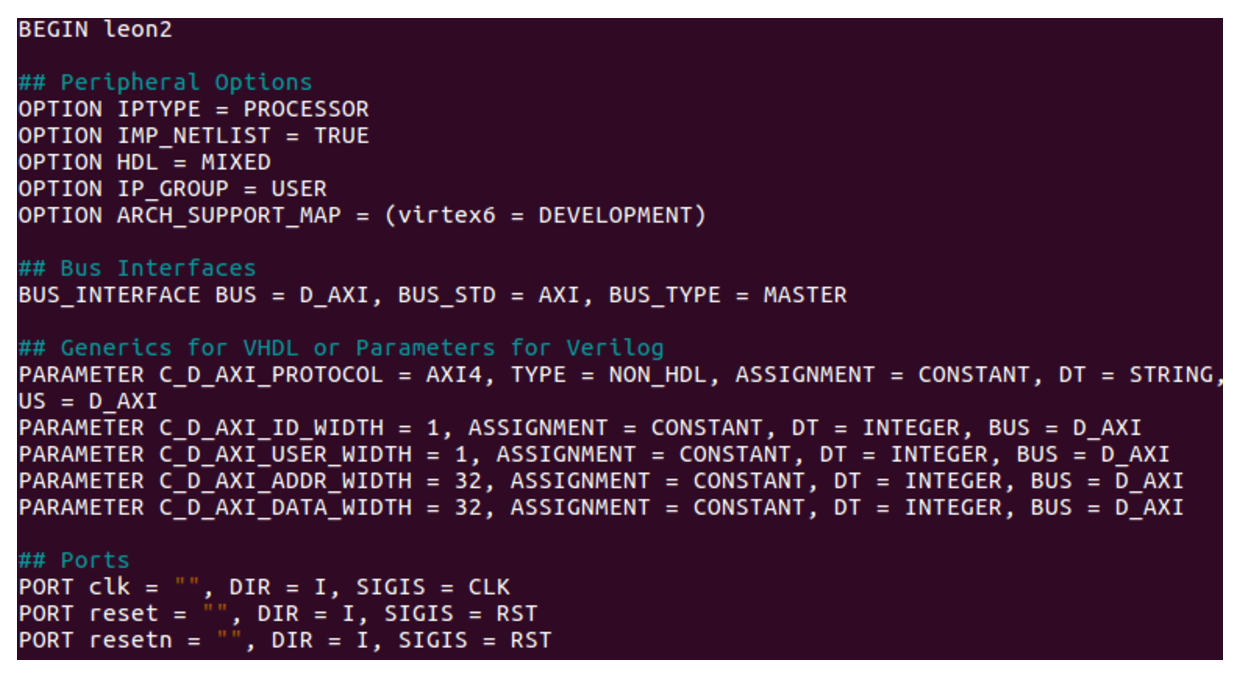
\includegraphics[width=0.9\textwidth]{fig/mpd.eps}
%\caption{Snapshot of leon2\_v2\_1\_0.mpd file}\label{fig-mpd}
%\end{figure}•


\end{enumerate}


\end{document}